\documentclass{article}
\usepackage[utf8]{inputenc}
\usepackage{polski}
\usepackage{geometry}
\usepackage{pdfpages}
\usepackage{pdfpages}
\usepackage{listings}
\usepackage{listingsutf8}
\usepackage{multirow}
\usepackage{siunitx}
\usepackage{multirow}
\usepackage{booktabs}
\usepackage{tabularx}
\usepackage{placeins}
\usepackage{pdflscape}

\geometry{
a4paper,
total={170mm,257mm},
left=20mm,
top=20mm
}
\newcolumntype{Y}{>{\centering\arraybackslash}X}
% \renewcommand\thesection{}
\lstset{%
literate=%
 {ą}{{\k{a}}}1
 {ę}{{\k{e}}}1
 {Ą}{{\k{A}}}1
 {Ę}{{\k{E}}}1
 {ś}{{\'{s}}}1
 {Ś}{{\'{S}}}1
 {ź}{{\'{z}}}1
 {Ź}{{\'{Z}}}1
 {ń}{{\'{n}}}1
 {Ń}{{\'{N}}}1
 {ć}{{\'{c}}}1
 {Ć}{{\'{C}}}1
 {ó}{{\'{o}}}1
 {Ó}{{\'{O}}}1
 {ż}{{\.{z}}}1
 {Ż}{{\.{Z}}}1
 {ł}{{\l{}}}1
 {Ł}{{\l{}}}1
}

\title{Technika Cyfrowa\\
Sprawozdanie - Przerzutniki i rejestry}
\author{Maciej Trątnowiecki}
\date{AGH, Semestr Letni, 2020}

\begin{document}
    \maketitle
    \section{Projekt przerzutnika RS}
        \subsection{Projekt układu}
            \begin{center}
                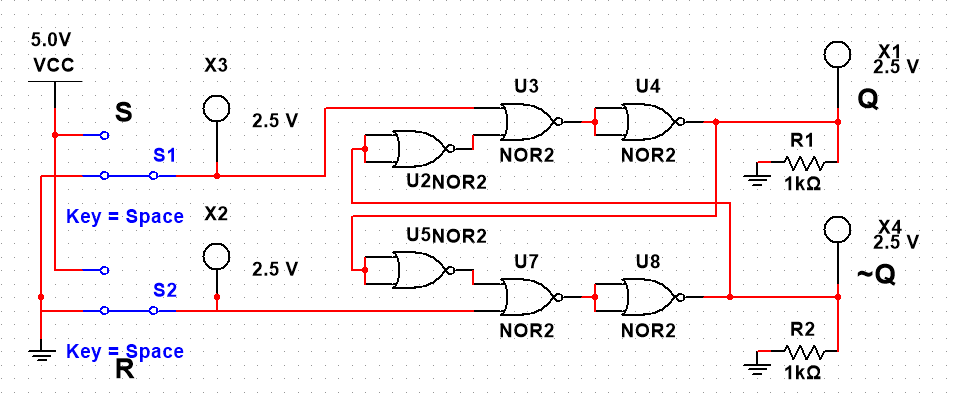
\includegraphics[width=18cm]{reports/img/Z2A_1.png}\\
            \end{center}
            Przerzutnik RS zbudowano w oparciu wyłącznie o bramki NOR. Układ realizuje funkcje opisaną poniższą tabelą prawdy. Do przetestowania układu wykorzystano probówki. 
            \begin{center}
                \begin{table}[ht]
                    \centering
                    \begin{tabular}{|c|c|c|c|}
                        \hline
                        S & R & $Q_n$ & $\neg$ Q\\
                        \specialrule{1pt}{1pt}{1pt}
                        0 & 0 & $Q_{n-1}$  & $\neg Q_{n-1}$\\
                        \hline
                        1 & 0 & 1 & 0\\
                        \hline
                        0 & 1 & 0 & 1\\
                        \hline
                        1 & 1 & - & -\\
                        \hline 
                    \end{tabular}
                    \caption{Tabela prawdy przerzutnika RS}
                    \label{tab:my_label}
                \end{table}
            \end{center}
        
        \subsection{Koncepcja budowy układu}
            W układzie wykorzystujemy sprzężenie zwrotne pomiędzy wyjściami układu (Q i zaprzeczone Q) oraz wejściami. Dodatkowe przełączniki NOR wykorzystujemy jako bramki NOT w celu dopasowania działania układu do standardowego przerzutnika RS. Gdy na wejście S podamy stan wysoki, a na wejście R niski, bramka U3 poda stan niski, zatem bramka U4 poda stan wysoki, przez co bramka U5 poda stan niski, czyli bramka U7 poda stan wysoki w efekcie czego dostajemy stan niski za bramką U8. Gdy następnie przestawimy oba wejścia układu w stan niski, bramka U3 dostanie na wejściu stan niski i stan wysoki (jako zaprzeczony stan wyjścia $\neg Q$), podając w efekcie stan niski, zaprzeczany przez bramkę U4. Z kolei Bramka U7 dostanie na wejściach dwukrotnie stan niski, dzięki czemu otrzymamy stan niski za bramką U8. Jak widzimy stan wyjść układu nie zmienił się - przerzutnik spełnił swoje zadanie. Przestawienie wejścia S w stan niski i wejścia R w stan wysoki spowoduje, że bramka U7 poda stan niski, zatem otrzymamy stan wysoki na wyjściu zanegowanego Q. Wtedy bramka U3 otrzyma dwa razy stan niski na wejściu, zatem otrzymany stan niski na wyjściu Q.\\ 
            Jak widać układ spełnia swoją funkcje.
            \begin{center}
                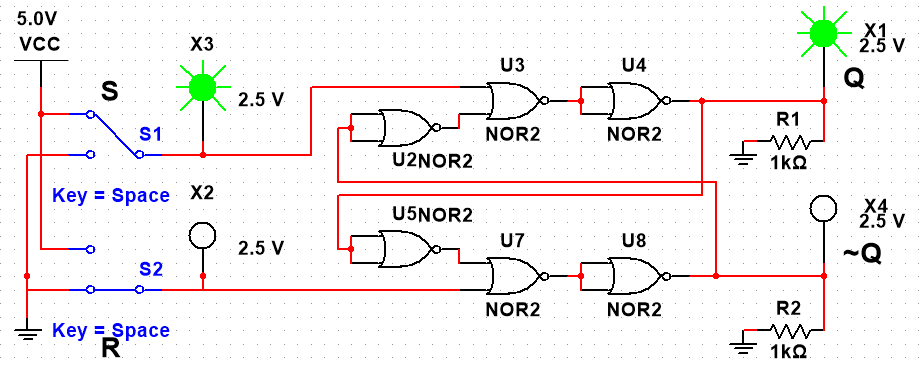
\includegraphics[width=18cm]{reports/img/Z2A_2.png}\\
            \end{center}

        \subsection{Wnioski}
            Udało nam się pokazać, że układ przerzutnika RS można łatwo skonstruować przy użyciu prostych i powszechnie dostępnych bramek logicznych. 
        
    \section{Budowa przerzutnika T}
        \subsection{Projekt układu}
            \begin{center}
                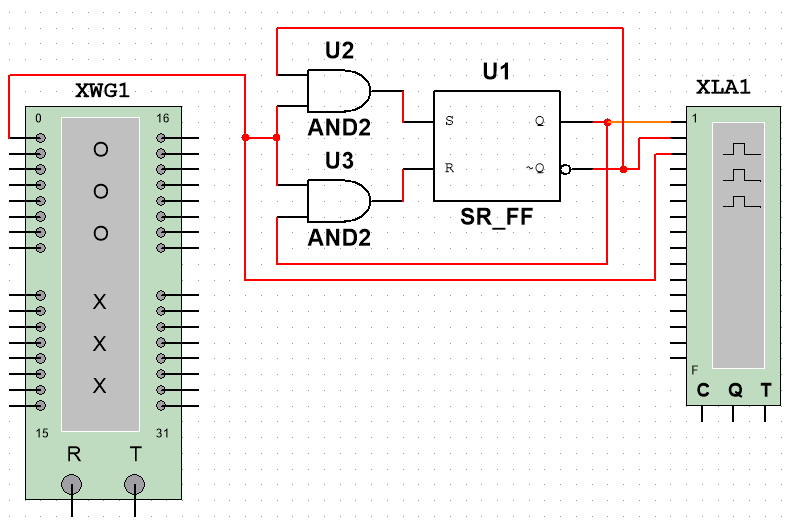
\includegraphics[width=18cm]{reports/img/Z2B_1.png}\\
            \end{center}
            Do budowy przerzutnika T wykorzystano przerzutnik RS oraz dwie bramki AND. Przerzutnik T posiada jedno wejście - T i dwa wyjścia - Q i zanegowane Q. Do wejścia T przerzutnika podłączono generator słów. Do wyjść przerzutnika podłączono analizator logiczny.\\ 
            Przerzutnik T realizuje funkcję opisaną poniższą tabelą stanów. 
            \begin{center}
                \begin{table}[ht]
                    \centering
                    \begin{tabular}{|c|c|c|}
                        \hline
                        T & $Q_n$ & $Q_{n+1}$\\
                        \specialrule{1pt}{1pt}{1pt}
                        0 & 0 & 0\\
                        \hline
                        0 & 1 & 1\\
                        \hline
                        1 & 0 & 1\\
                        \hline
                        1 & 1 & 0\\
                        \hline 
                    \end{tabular}
                    \caption{Tabela prawdy przerzutnika T}
                    \label{tab:my_label}
                \end{table}
            \end{center}
        
        \subsection{Koncepcja budowy układu}
            Ponieważ w konstrukcji przerzutnika chcemy wykorzystać przerzutnik RS, zestawmy tabele prawdy przerzutnika T ze stanami wejść przerzutnika RS dla odpowiadających im wartości wyjść. 
            \begin{center}
                \begin{table}[ht]
                    \centering
                    \begin{tabular}{|c|c|c|c|c|}
                        \hline
                        T & $Q_n$ & $Q_{n+1}$ & S & R\\
                        \specialrule{1pt}{1pt}{1pt}
                        0 & 0 & 0 & 0 & - \\
                        \hline
                        0 & 1 & 1 & - & 0\\
                        \hline
                        1 & 0 & 1 & 1 & 0\\
                        \hline
                        1 & 1 & 0 & 0 & 1\\
                        \hline 
                    \end{tabular}
                    \caption{Tabela prawdy przerzutnika T z odpowiadającymi jej stanami wejść przerzutnika RS}
                    \label{tab:my_label}
                \end{table}
            \end{center}
            Korzystając z tak przygotowanej tabeli prawdy, możemy dopasować bramki logiczne dla wejść przerzutnika RS. W swoim układzie wykorzystałem dwie bramki AND, jedna z nóg każdej z bramek podłączona jest do wejścia T układu, drugą łącze z odpowiednim wyjściem układu. 
        
        \subsection{Sposób działania układu}
            Tak przygotowany układ przetestowałem za pomocą analizatora logicznego, upewniając się że poprawnie realizuje funkcje zdefiniowaną w tabeli prawdy. 
            \begin{center}
                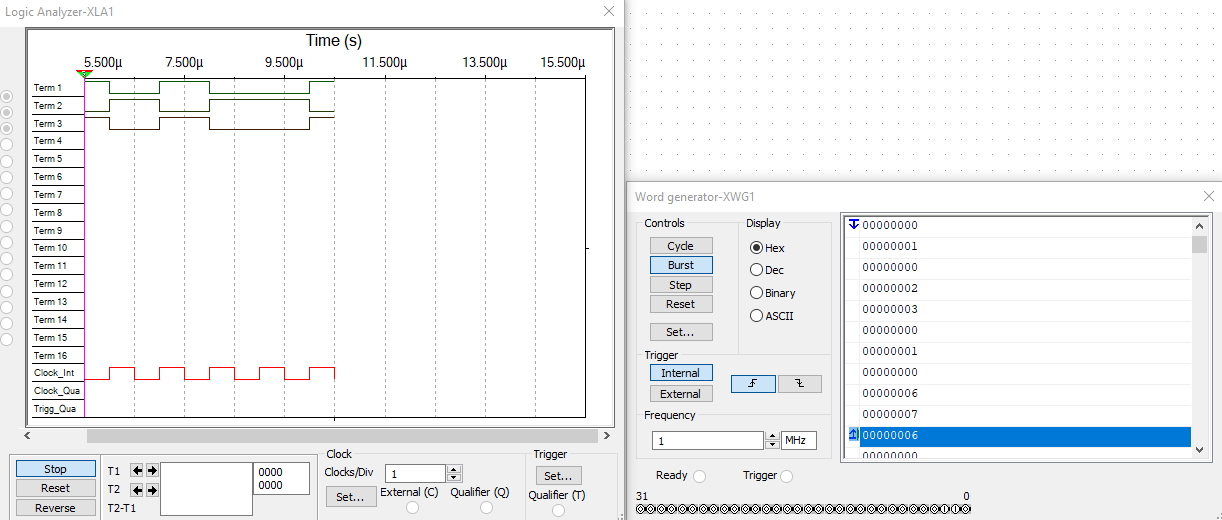
\includegraphics[width=18cm]{reports/img/Z2B_2.png}\\
            \end{center}

            
        \subsection{Wnioski}
            Przy użyciu prostych bramek logicznych możemy przeprowadzać konwersję pomiędzy poszczególnymi typami przerzutników.
    
    \section{Układ szeregowy nadajnika - odbiornika}
        \subsection{Projekt układu}
            \begin{center}
                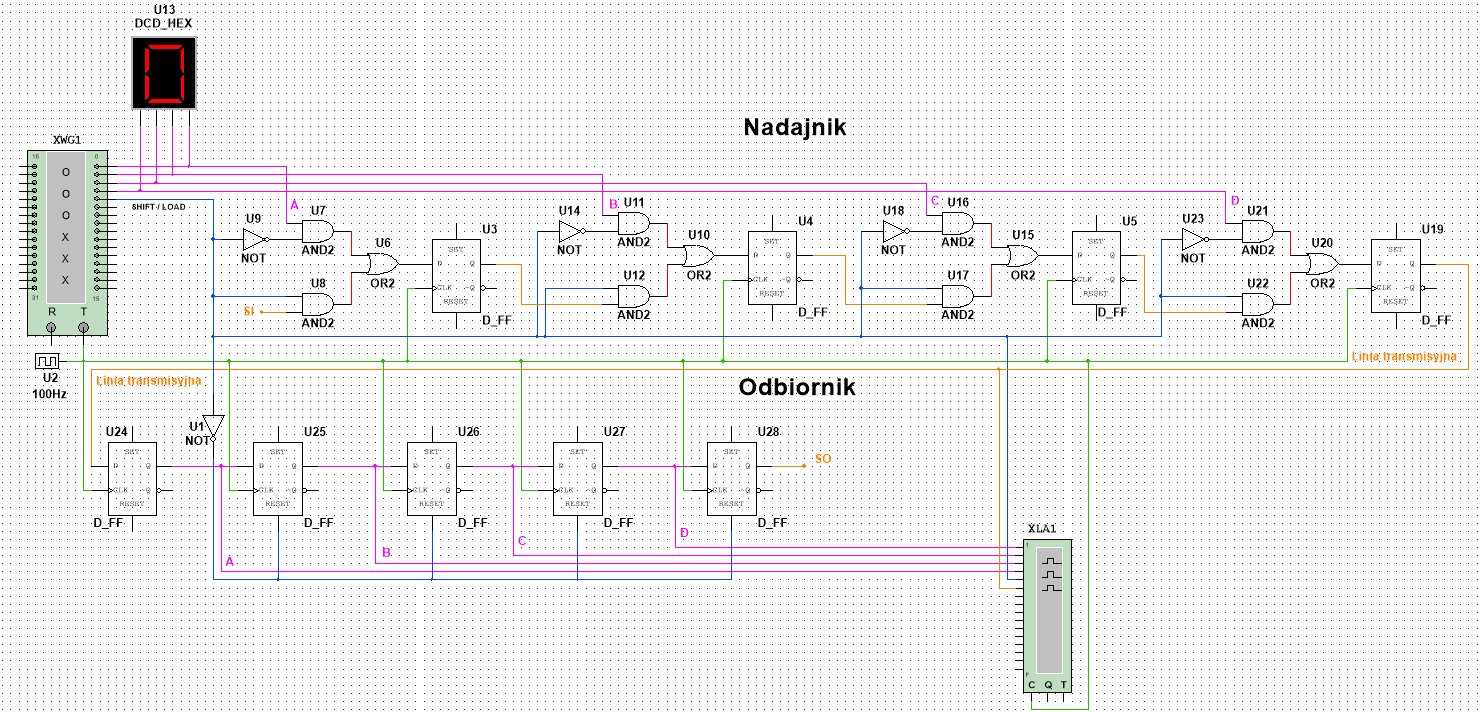
\includegraphics[width=18cm]{reports/img/Z2C_1.png}\\
            \end{center}
            Rejestry nadajnika i odbiornika zbudowałem z wykorzystaniem przerzutników D. Generator słów podaje na wejście układu nadajnika czterobitową liczbę (jako sygnał równoległy). Następnie podaje sygnał przesunięcia. Nadajnik przekazuje liczbę jako sygnał szeregowy. Układ odbiornika odczytuje sygnał szeregowy do sygnału równoległego. Jego wyjścia połączone są z analizatorem logicznym. 
            
        \subsection{Sposób działania układu}
            \begin{center}
                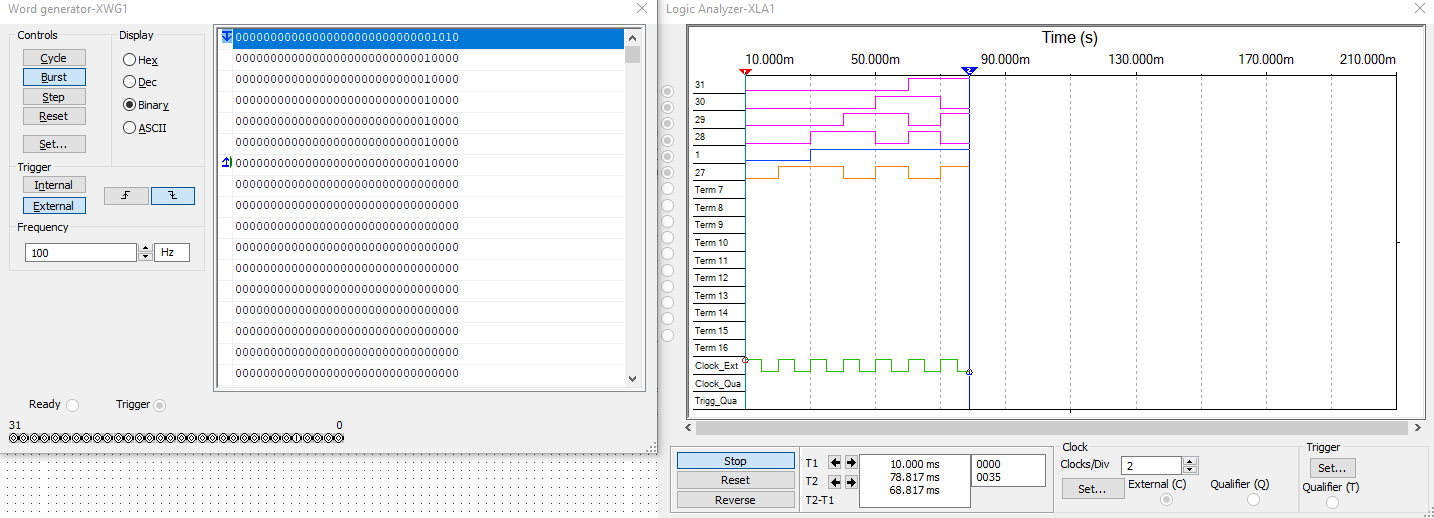
\includegraphics[width=18cm]{reports/img/Z2C_2.png}\\
            \end{center}
            
        \subsection{Wnioski}

\end{document}
